\section{Segunda pregunta de investigación}
\label{sec:RQ2}

\noindent\fbox{%
\parbox{\dimexpr\textwidth-2\fboxsep-2\fboxrule\relax}{%
\textbf{RQ2} ¿Cuales métricas de código fuente son buenas predictoras de errores y en que tipo de métrica (archivo, clase,
método) proporciona mejores resultados?%
}%
}
\vspace{12pt}

Se implementaron 6 algoritmos de selección de características (\ref{fig:Flow}) y al terminar cada etapa, se registran todos los resultados pertinentes, incluyendo las métricas seleccionadas por cada algoritmo y los distintos valores de rank y $\beta$ utilizados.

Posteriormente, se realizó un análisis de la frecuencia de aparición de cada métrica en todos los algoritmos de selección. Ordenando los resultados desencendentemente por la suma de la frecuencia de aparición de cada métrica en los seis esquemas de selección utilizados. Como resultado, se identificaron las 23 métricas con mayor frecuencia de aparición, cuyos detalles se ilustran en \ref{fig:sum_frecuency}.

\begin{figure}[H]
	\centering
	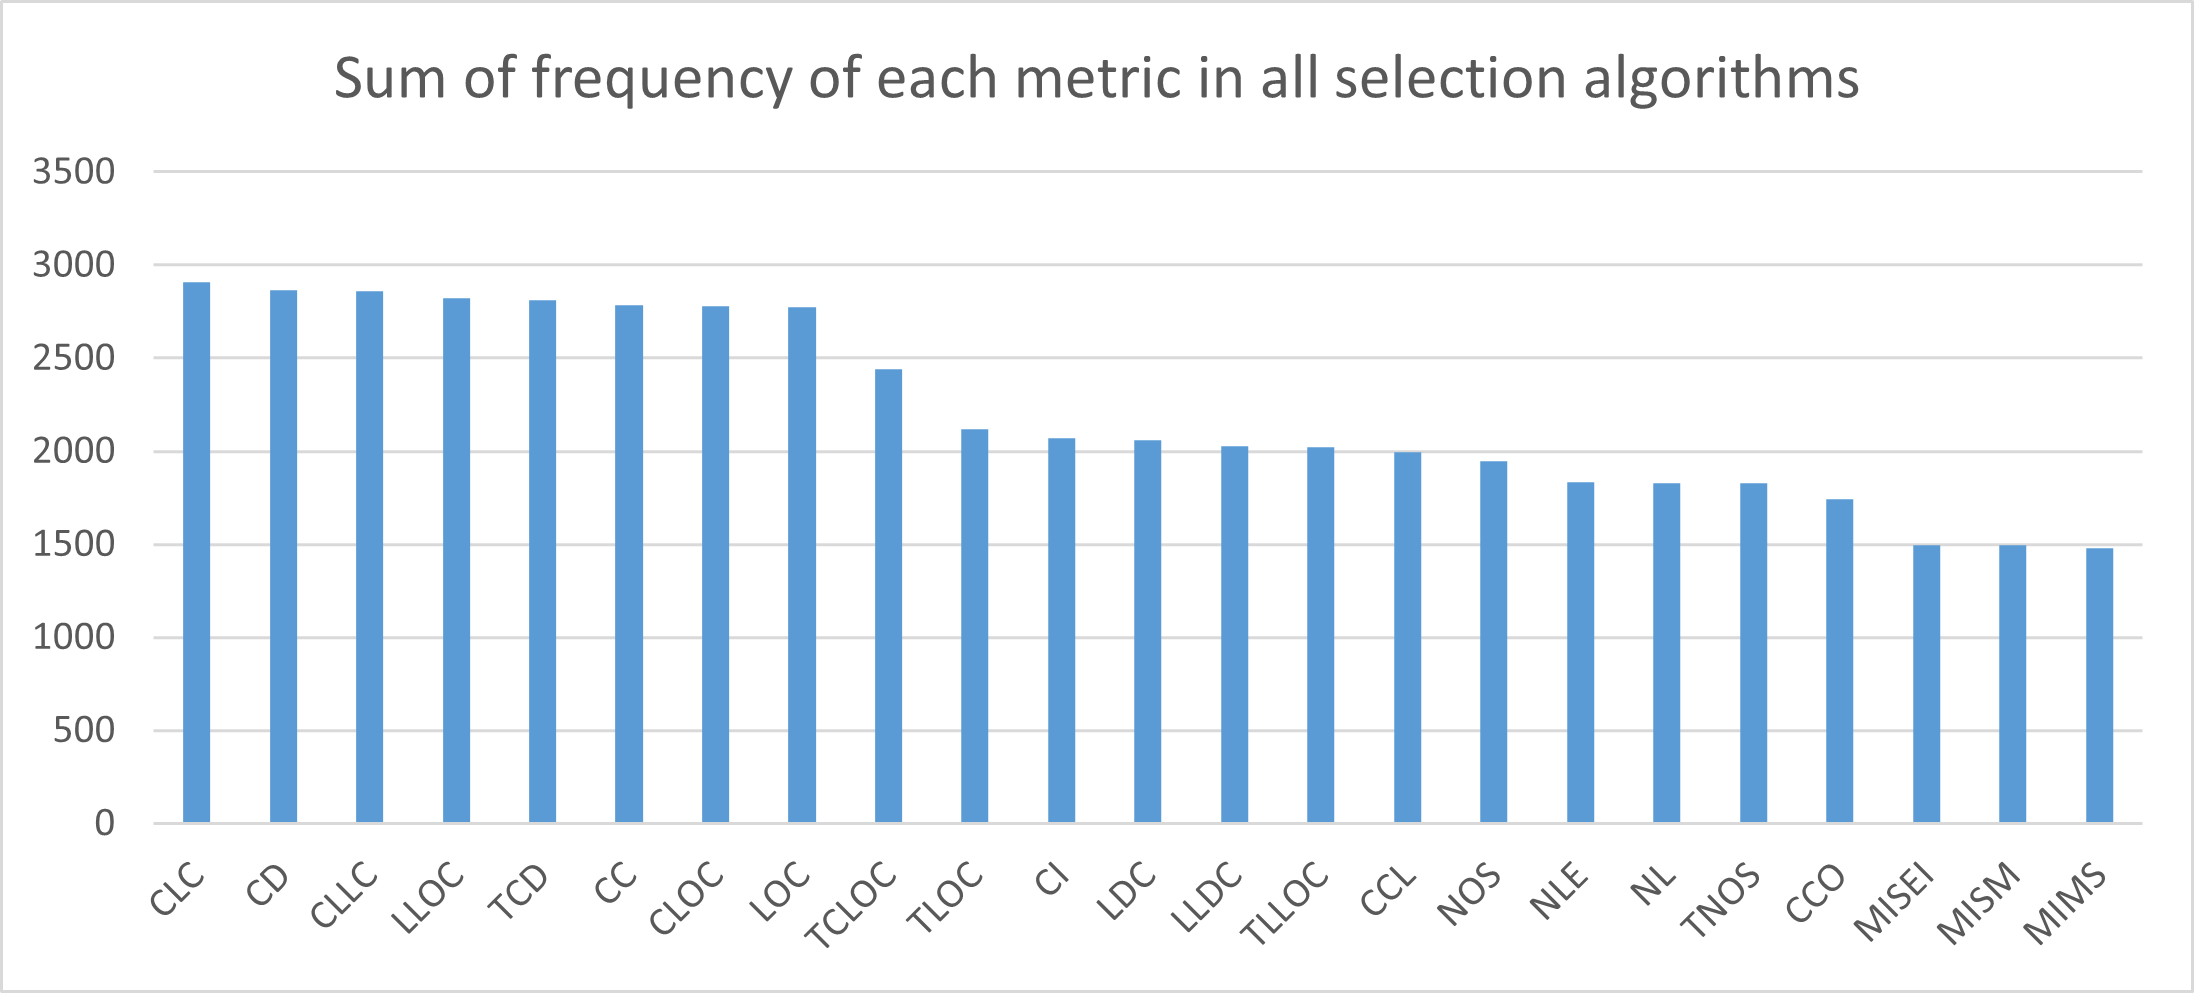
\includegraphics[scale=0.9]{chapters/chapter3/Sections/Research Questions/sections/RQ2/img/frec_all.png} %Change the figure name 
	\setstretch{1} %Interlineado 1
	\captionsetup{labelsep=period, labelfont=bf}
	\caption[Suma de la frecuencia de aparición de cada métrica en todos los algoritmos de selección]{Suma de la frecuencia de aparición de cada métrica en todos los algoritmos de selección} %[Se muestra en el índice]{Se muestra en el pie de figura}
	\label{fig:sum_frecuency}
\end{figure}


En la figura \ref{fig:frecuencyby}, se observa un patrón consistente: en promedio, los algoritmos de selección que incorporan el algoritmo de SU en su etapa de control de redundancia tienden a resultar en un menor número de características seleccionadas, en comparación con aquellos que utilizan la COS.

\begin{figure}[H]
	\centering
	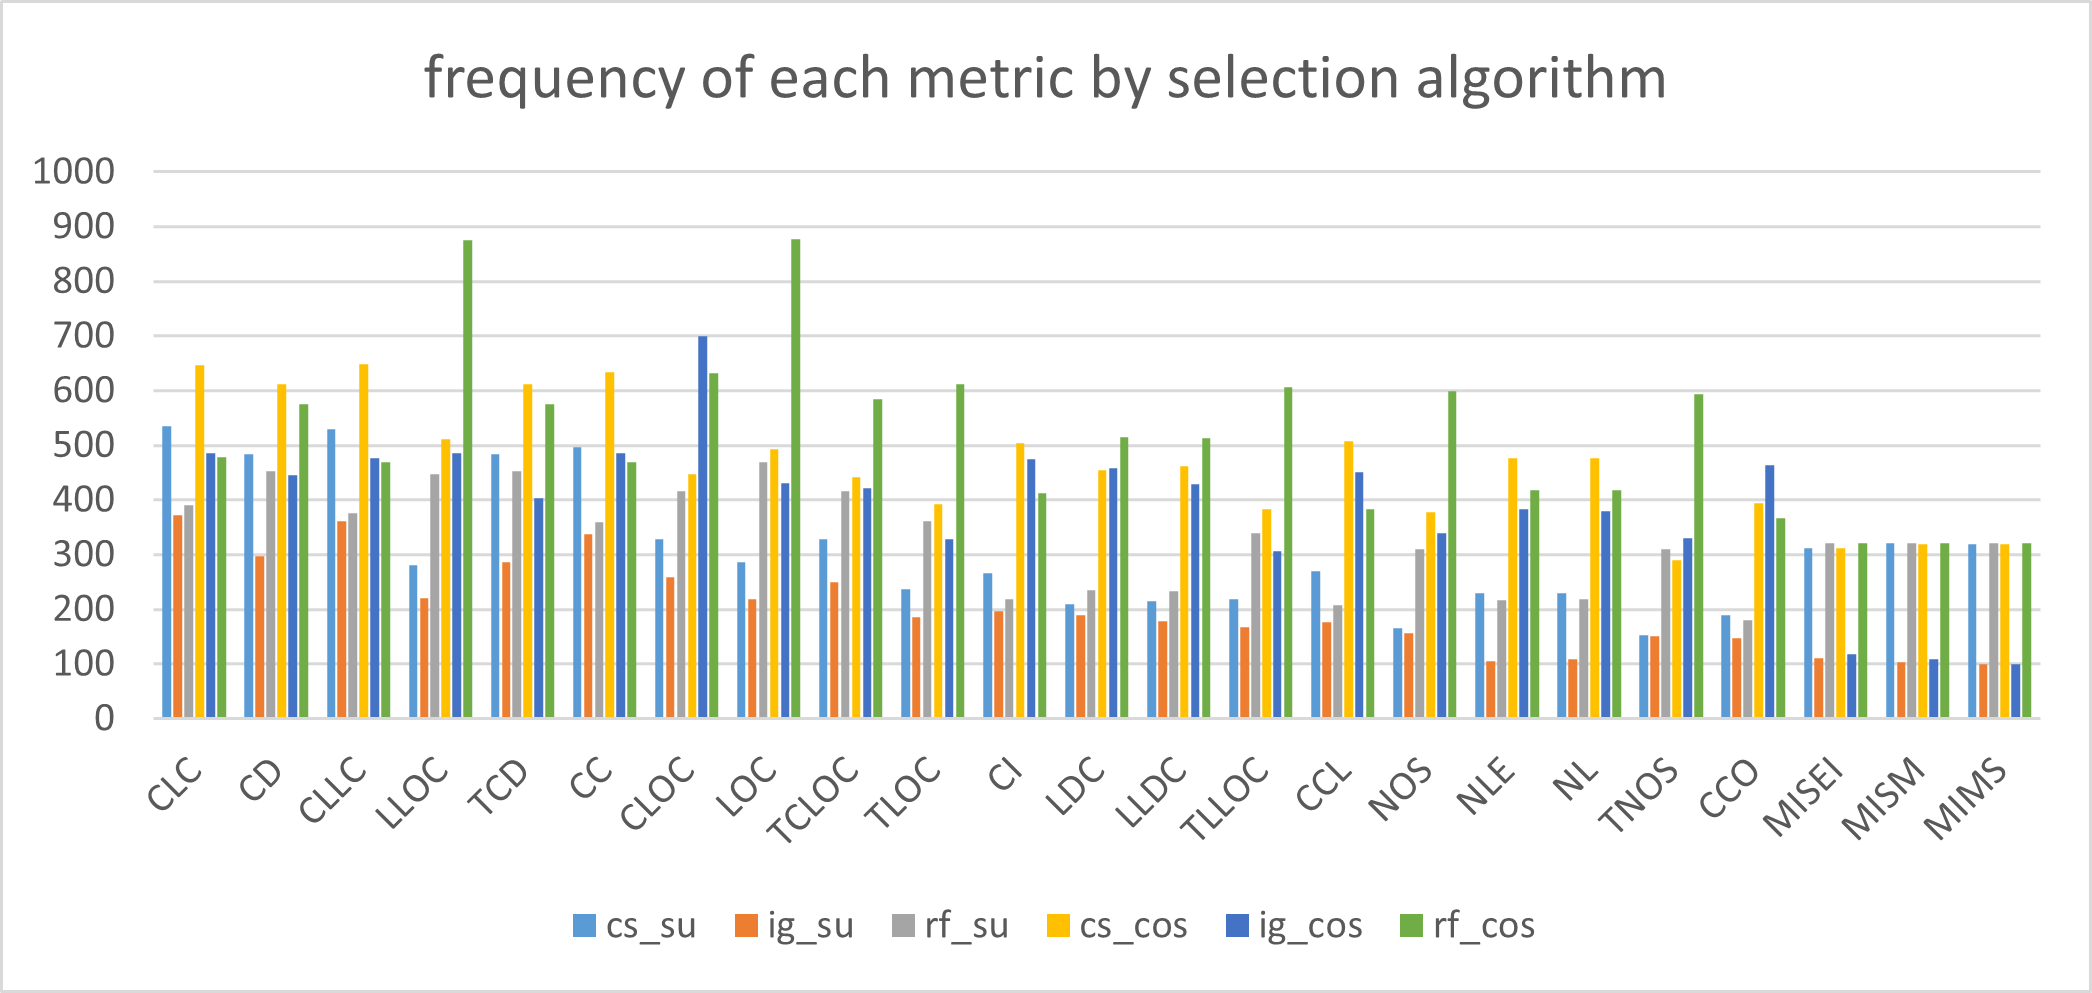
\includegraphics[scale=0.9]{chapters/chapter3/Sections/Research Questions/sections/RQ2/img/frec_by.png} %Change the figure name 
	\setstretch{1} %Interlineado 1
	\captionsetup{labelsep=period, labelfont=bf}
	\caption[Frecuencia de cada métrica \(\beta\) y algoritmo de selección]{Frecuencia de cada métrica \(\beta\) y algoritmo de selección}
 %[Se muestra en el índice]{Se muestra en el pie de figura}
	\label{fig:frecuencyby}
\end{figure}



En la la tabla \ref{table:selected_metrics} se muestra las métricas de código y la tabla \ref{table:cloneMetrics} separa las métricas de clone \cite{ferenc_automatically_2020} las cuales son calculadas a nivel de método y clase.

% Please add the following required packages to your document preamble:
% \usepackage{graphicx}
\begin{table}[H]
{
\fontsize{6pt}{6pt}\selectfont
\captionsetup{labelsep=period, labelfont=bf}
\caption{\label{table:selected_metrics} Ranking de las 15 mejores métricas de código seleccionadas}
\centering
\resizebox{\textwidth}{!}{%
\begin{tabular}{lllll}
\toprule
Abreviation & Full name                                   & Method & Class & File \\
\midrule
CD           & Comment Density                             & X      & X     &      \\
LLOC         & Logical Lines of Code                       & X      & X     & X    \\
TCD          & Total Comment Density                       & X      & X     &      \\
CLOC         & Comment Lines of Code                       & X      & X     & X    \\
LOC          & Lines of Code                               & X      & X     & X    \\
TCLOC        & Total Comment Lines of Code                 & X      & X     &      \\
TLOC         & Total Lines of Code                         & X      & X     &      \\
TLLOC        & Total Logical Lines of Code                 & X      & X     &      \\
NOS          & Number of Statements                        & X      & X     &      \\
NLE          & Nesting Level Else-If                       & X      & X     &      \\
NL           & Nesting Level                               & X      & X     &      \\
TNOS         & Total Number of Statements                  & X      & X     &      \\
MISEI        & Maintainability Index (SEI version)         & X      &       &      \\
MISM         & Maintainability Index (SourceMeter version) & X      &       &      \\
MIMS         & Maintainability Index (Microsoft version)   & X      &       &   \\
\bottomrule
\end{tabular}%
}
}

\end{table}

Como se evidencia en la Tabla \ref{table:selected_metrics}, las métricas seleccionadas prioritariamente corresponden al nivel de método, seguidas por las métricas a nivel de clase y, finalmente, las de archivo. Es importante destacar que la cantidad de métricas disponibles a nivel de archivo es considerablemente menor en comparación con las de nivel de método y clase. Paralelamente, según lo indicado en la Tabla \ref{metrics-table}, solo tres métricas - CLOC, LOC y LLOC - están presentes en los tres niveles mencionados. Estas métricas fueron seleccionadas entre las más contribuyentes a los modelos predictivos. Esto subraya la relevancia y eficacia de dichas métricas en la predicción de errores.

\begin{table}[h]
\centering{
\captionsetup{labelsep=period, labelfont=bf}
\caption{Best clone metrics selected}
\begin{tabular}{ll}
\toprule
Abreviatura & Nombre completo                        \\
\midrule
CLC          & Clone Line Coverage              \\
CLLC         & Clone Lines of Code              \\
CC           & Clone Coverage                   \\
CI           & Clone Instances                  \\
LDC          & Lines of Duplicated Code         \\
LLDC         & Logical Lines of Duplicated Code \\
CCL          & Clone Classes        \\
\bottomrule
\end{tabular}%


\label{table:cloneMetrics} 
}
\end{table}


En la tabla \ref{table:metric_cero_varia} se muestran las métricas que no tienen variación en sus datos, aquellas que contengan aproximadamente un 95\% o más de sus datos con un valor constante. 

 \begin{table}[H]
{
\fontsize{10pt}{10pt}\selectfont
\captionsetup{labelsep=period, labelfont=bf}
\caption{Características con poca variación en sus valores}
\label{table:metric_cero_varia}
\centering{
\begin{tabular}{llll}
\toprule
\textbf{Nombre   completo}          & \textbf{Valores} & \textbf{Cantidad} & \textbf{Total} \\
\midrule

WarningCritical                     & 0                & 159078            & 100\%          \\
\hline
Unnecessary and Unused   Code Rules & 0                & 159077            & 99.99\%        \\
                                    & 1                & 1                 & 0.01\%         \\
                                    \hline
Java Logging Rules                  & 0                & 159078            & 100\%          \\
\hline
Import Statement Rules              & 0                & 159007            & 99.95\%        \\
                                    & 1-5           & 71                & 0.15\%         \\
                                    \hline
Migration15 Rules                   & 0                & 150949            & 94.88\%        \\
                                    & 1-6,15           & 1171              & 0.73\%         \\
                                    \hline
WarningMinor                        & 0                & 159078            & 100\%          \\
\hline
Migration Rules                     & 0                & 159078            & 100\%          \\
\hline
Migration13 Rules                   & 0                & 159078            & 100\%          \\
\hline
Migration14 Rules                   & 0                & 159078            & 100\%          \\
\hline
MigratingToJUnit4 Rules             & 0                & 158991            & 99.94\%        \\
\hline
                                    & 1-4,6            & 87                & 0.06           \\
                                    \hline
JavaBean Rules                      & 0                & 159078            & 100\%          \\
\hline
Jakarta Commons Logging   Rules     & 0                & 155047            & 97.46\%        \\
                                    & 1-22           & 4039              & 2.54\%         \\
                                    \hline
JUnit Rules                         & 0                & 157826            & 99.21\%        \\
                                    & 01-9          & 1252              & 0.79\%         \\
                                    \hline
Finalizer Rules                     & 0                & 156912            & 98.63\%        \\
                                    & 1-81           & 2166              & 1.37\%         \\
                                    \hline
Empty Code Rules                    & 0                & 159054            & 99.98\%        \\
                                    & 1                & 24                & 0.02\%         \\
                                    \hline
Design Rules                        & 0                & 157537            & 99.03\%        \\
                                    & 1-15           & 1541              & 0.96\%         \\
                                    \hline
Comment Rules                       & 0                & 159078            & 100\%          \\
\hline
Clone Implementation Rules          & 0                & 159078            & 100\%          \\
\hline
Brace Rules                         & 0                & 159035            & 99.97\%        \\
\hline
                                    & 01-2           & 43                & 0.027\%        \\
                                    \hline
TNOS                                & 0                & 159077            & 99.99\%        \\
\hline
                                    & 1                & 1                 & 0.01          
\\\bottomrule
\end{tabular}
}
\captionsetup{labelsep=period, labelfont=bf}



}

\end{table}

De acuerdo con los análisis presentados en las tablas \ref{description-table} y \ref{table:metric_cero_varia}, se observa que, a excepción de la métrica TNOS, todas las demás métricas relacionadas con la violación de reglas presentan poca variación en sus datos (ver tabla \ref{table:smell_metrics}). Este patrón sugiere que dichas métricas podrían no ser particularmente relevantes para el proceso de predicción de errores en el contexto estudiado.

\textit{Advertencia sobre un posible artefacto de conteo.} Una explicación alternativa, no excluyente, para la alta frecuencia de selección de CLOC, LOC y LLOC es un artefacto de conteo: al ser las únicas tres métricas disponibles en los tres niveles de granularidad, tienen estructuralmente el triple de oportunidades de ser seleccionadas que una métrica exclusiva de un solo nivel, y el doble que una disponible en dos niveles. Los datos actuales no permiten distinguir, sin reprocesar los registros de selección normalizando por nivel de granularidad, entre valor predictivo genuino y este efecto de oportunidad; esta verificación se declara como trabajo futuro (Capítulo \ref{cap:conclusion}) y como amenaza a la validez de constructo (Capítulo \ref{cap:discusion}).

\noindent\fbox{%
\parbox{\dimexpr\textwidth-2\fboxsep-2\fboxrule\relax}{%
\textbf{Respuesta RQ2}
   Entre las métricas con mayor contribución se encuentran aquellas calculables en los tres niveles: método, clase y archivo, específicamente CLOC, LOC y LLOC, aunque parte de su preeminencia puede deberse a que tienen más oportunidades de ser seleccionadas. No obstante, según se detalla en la Tabla \ref{table:selected_metrics}, las métricas de código más relevantes para los modelos empleados en la selección de características son, en orden de importancia, aquellas a nivel de método, clase y archivo, respectivamente. En resumen, las métricas más relevantes para la predicción de errores son las métricas de código fuente, seguidas por las métricas de clonación de código, mientras que las métricas de violación de reglas (\textit{code smells}) quedan prácticamente fuera, con la excepción de TNOS.
}%
}
\vspace{12pt}